\chapter{Event Simulation and Object Reconstruction}\label{chapter:data-mc}
After triggered events from the CMS experiment have been read out, the reconstruction of the physics objects which the detector signals correspond to is performed.
Monte Carlo (MC) simulations, which provide a detailed, precise and realistic description of the expected SM and potential BSM processes, form an essential component of performing any physics analysis.
MC is used for optimising signal extraction strategies and for 

 
The event simulation and objection reconstruction algorithms which are relevant to the single top physics search presented in this thesis are discussed in this chapter.

\section{Event Simulation}\label{sec:sim}
As MC simulation is meant to provide a realistic description of physics processes, both accurate modelling of these processes and a detailed understanding of how physical processes interact with the CMS detector are required to produce events in the same format as raw proton-proton collision data prior to undergoing the same reconstruction process.


%In hadron collisions,
%
%As model hadron collision we need
%As a hadron contains not jist sea of gluons and quarks from the continuous gluon splitting inside it in addition to its constituent valence quarks, 
%
%For the accurate modelling of hadron collisions, knowledge of the internal structure of each hadron 
%
%The inability to directly measure 
%Another difficulty arises from colour confinement preventing 
% the accurate modelling 
%
%The 
%continual gluon splitting inside a hadron results in it  
%As colour confinement results in a hadron containing not only its constituent valence quarks but also a sea of gluons and quarks from the continuous gluon splitting inside
%
%Consequently, as a hadron consists of not only its constituent valence quarks but also a  it~\cite{coughlan2006ideas,evenish2004deep}.
%The first evidence of the 
%The probing of the proton through Deep Inelastic Scattering (DIS) is used to experimentally determine how the number 
%
%
%
%each constituent valence quark within a hadron does not possess an equal fraction of the hadron's momentum due to the 
%Given that 
%As colour confinement prevents a hadron's constituent elements being ..., their internal structure is probed  using 
%\editComment{PDFs and DIS to be added}
%
%PDFs are an essential component of modelling hadron collisions
%
%~\cite{evenish2004deep} - DIS

The simulation of events is a four stage process: generation (GEN), simulation (SIM), digitisation (DIGI) and

 reconstruction (RECO).

The initial GEN stage involves the use \emph{event generators} to simulate the proton-proton interactions and the resultant physics processes~\cite{Buckley:2011ms,Hoche:2014rga}.
The first stage of this is the modelling of the colliding protons and the hard scattering of their constituent partons, which involves the use Parton Distribution Functions (PDFs) to assign fractions of the proton's momentum to the partons and perturbation theory to compute the Matrix Elements (ME) of the Feynman diagrams for the QCD and electroweak processes involved.
The second stage models resultant Parton Showers (PS) through an iterative process until the infrared cutoff scale for the shower is reached and perturbation theory no longer applies.
The remaining particles undergo hadronisation using non-perturbative modelling process.
The various event generators used in the production of MC samples used in this thesis are discussed in Section~\ref{subsec:eventGenerators}.

Following the GEN stage, the SIM stage involves passing the GEN output through a complete simulation of the CMS detector that has been with the GEANT4 program~\cite{geant4,Lefebure:1999wja}.
This process models particle interactions and decays and the propagation of particles through the detector, the effects of solenoidal field and detector material.
The DIGI stage uses the SIM output to produce the detector's electronics response, which then undergoes the same RECO process that data does, as described in Section~\ref{sec:reco}.

The inelastic proton-proton interactions, typically called pileup (\PU), which occur both within and adjacent to the event's bunch crossing, referred to as \emph{in-time} and \emph{out-of-time} \PU  respectively, also require modelling in simulation.
Simulated \PU however, does not adequately describe observed \PU in data.
Therefore, the reweighting of the simulated samples is required and is discussed in Section~\ref{subsec:puSF}.

\subsection{Event Generators}\label{subsec:eventGenerators}
A number of event generators are used by CMS to produce the MC simulation samples used to describe the expected processes produced.
Whilst there are several general-purpose event generators which can describe an event from the initial hadron collision to final state particles, they are typically used in conjunction with generators that specialise in a specific physics aspect (\ie ME calculations or PS simulation) or process (\eg tau decays) in order to provide a complete event.
Perturbative calculations of the MEs of the QCD and electroweak processes are done, where possible, to Next-To-Leading Order (NLO) in order to both enable precision measurements to be made and to accurately model processes with many distinct high energy jets.

The MC samples used to model the background and signal processes for the analysis presented in this thesis were simulated using the following generators:

\begin{itemize}
%\item \textbf{Madgraph} - Madgraph~\cite{Alwall:2011uj} is a package which performs tree-level perturbativecalculations to produce matrix elements at Leading Order (LO) for processes %such as decays and 2 $\rightarrow$ n scatterings through evaluating the ME for a given phase space point for all the Feynman diagrams produced.
\item \textbf{Madgraph} - Madgraph~\cite{Alwall:2011uj} is a package which performs tree-level perturbativecalculations to produce matrix elements at Leading Order (LO) for processes through evaluating the ME for a given phase space point for all the Feynman diagrams produced.
\item \textbf{aMC@NLO} - aMC@NLO~\cite{Alwall:2014hca} is a package that considers tree-level and one-loop Feynman diagrams to produce matrix elements at NLO.
Considering the constructive and destructive interferences which result from considering both the leading and higher order cross section terms results in positively and negatively weighted events.
These negatively weighted events are not simply discarded as they are required to correctly simulate the NLO cross section by applying a scale factor, $SF^{NLO}$, which considers the ratio of the total number of events to the effective number of events (\ie the difference in positively and negatively weighted events) in the sample and the sign of an individual event's weighting:
\begin{equation}
SF^{NLO} = \frac{N^{postive events} + N^{negative events}}{N^{postive events} - N^{negative events}} \times \frac{|event weight|}{event weight} \;
\end{equation}

\item \textbf{POWHEG} - The Positive Weight Hardest Emission Generator (POWHEG)~\cite{Alioli:2010xd} is a framework that interfaces NLO ME calculations with PS generators.
As its name suggests, POWHEG produces the hardest emission first through using the exact NLO ME and produces only positively weighted events.
The latter is achieved by interfacing to a PS generator which order emissions by \pT or allows for the use of a $p_{T}$-veto to reject subsequent emissions, avoiding double counting such emissions and the need for negative weights.
\editComment{Worth mentioning angular ordered generators? Wary of needing to defend that several levels beyond what is written.}
\item \textbf{PYTHIA} - PYTHIA~\cite{Sjostrand:2014zea} is a general-purpose generator which capable of taking the output of a ME event generator and perform the parton showering and hadronisation to produce the full event. For all of the MC samples considered in Section~\ref{sec:samples} for the analysis presented, PYTHIA 8 is used to develop the samples from their ME event generator output into a full event.
\end{itemize}

\section{Object Reconstruction}\label{sec:reco}
Using the readouts of all of the CMS sub-detectors, a full reconstruction of the triggered physics event is undertaken.
This process involves the \emph{Particle Flow} (PF) algorithm which combines the complementary information from each of the CMS sub-detectors, known as \emph{elements}, to provide an optimal reconstruction and identification of all of the stable particles present in the event~\cite{CMS:2009nxa,CMS:2010eua,CMS-PRF-14-001}.
Using these reconstructed particles, additional objects such as b-jets and missing transverse energy can also be constructed.

\subsection{Charged Particle Tracks}\label{subsec:tracks}
As the charged particles produced from the proton-proton collisions traverse the silicon tracker, they interact with it and leave energy deposits known as \emph{hits}.
These hits are used to reconstruct the particles' trajectories through multiple iterations of the Combinatorial Track Finder (CTF) algorithm, which is based off combinatorial Kalman Filtering~\cite{Chatrchyan:2014fea,Fruhwirth:1987fm}.

The steps of each iteration of the CTF algorithm are:
\begin{itemize}
\item \textbf{Seed generation:} Initial track candidates are formed from two or three hits to provide a first estimate of the tracks' helix parameters.
\item \textbf{Track Finding:} A combinatorial Kalman Filter then builds a candidate by adding hits from successive layers which are compatible with the extrapolated trajectory, which is updated with the addition of each subsequent hit, taking into account the hit's position, uncertainty and material traversed.
\item \textbf{Track Fitting:} The initial estimate of a built track's parameters is improved upon with the Kalman Filter performing two passes, the first from the innermost layer outwards and the second from the outermost inwards.
This approach minimises the bias in determining and discarding which hits are incorrectly associated with the track.
\item \textbf{Track Selection:} Quality criteria, such as $\chi^{2}$, the number of layers with hits and compatibility, are used to reject \emph{fake} tracks which are not associated with a charged particle.
\end{itemize}

Up to six iterations of the CTF are performed, with selected tracks' hits removed from consideration by subsequent iterations.
Whilst initial four iterations use seeds exclusively from the pixel tracker, the last two iterations use seeds from the strip tracker to enable a high track reconstruction efficiency for those originating outside the pixel or those which did not leave any hits in the pixel tracker.

\subsection{Primary Vertices}\label{subsec:vertices}
The reconstructed tracks are subsequently used to reconstruct the positions where the proton-proton collisions occurred, known as the \emph{primary vertices}~\cite{Speer:2006mh,Chatrchyan:2014fea}.
Initially tracks are required to be consistent with originating promptly from the interaction region, namely having a small transverse impact parameter, a minimum number of hits in the pixel and strip trackers and a low normalised $\chi^{2}$.
Such tracks are then clustered along the z-axis at their point of closest approach to the beamspot using a deterministic annealing algorithm	~\cite{Kenneth:1998i}, with these vertex candidates being used as input to an adaptive vertex filter~\cite{Fruhwirth:2007hz} to provide 3D position fits, uncertainties and variables such as the number of degrees of freedom to discriminate against fake vertices.
Out of these resultant primary vertex candidates, the one with the greatest scalar transverse momentum is considered as the \emph{primary vertex}, with the rest being considered \PU vertices.
Displaced vertices, such as those from heavy hadrons, are reconstructed during later reconstruction stages.

\subsection{Calorimeter Energy Clusters}\label{subsec:clustering}
The energy deposited by particles in the calorimeters is independently clustered in each sub-detector, except for the HF where each large cell can give rise to one cluster, to determine the energy and direction of the particles~\cite{CMS:2009nxa}.

The clustering algorithm consists of three steps:
\begin{itemize}
\item \textbf{Cluster seeding} - local cells' energies above a thresholds are considered as seeds.
\item \textbf{Clustering} - adjacent cells are summed together to form topological clusters.
\item \textbf{Energy threshold} - if the energy of the cluster is greater than two standard deviations of the electronics noise (80\MeV in the EB, up to 300\MeV in the EE, and 800\MeV in the HCAL), the cluster is accepted.
\end{itemize}

\subsection{Particle Flow Algorithm}\label{subsec:PF}
Through combining the calorimeters' energy clusters and charged particle tracks from the tracker and muon systems, the Particle Flow algorithm is able to use all the available information from an event to reconstruct and identify all stable particles in an event with far superior results than if each sub-detector were used individually.

The initial stage of the process involves associating charged particle tracks to energy clusters from the ECAL and HCAL sub-detectors.
Tracks are extrapolated from the last hit in the tracker to the typical shower profiles in the calorimeters, and if the particles' expected positions in the calorimeters are within the clusters' boundaries, these elements are linked together.

These linked elements are used by the Particle Flow algorithm to sequentially reconstruct and identify PF particles, removing classified elements from further consideration, with the least ambiguous or cleanest objects reconstructed first, followed by progressively more difficult objects which can be constrained by previous ones.

This is done in the following order: 
\begin{itemize}
\item muons are reconstructed, as described in Section~\ref{subsec:objReco-muons}.
\item electrons and associated Bremsstrahlung photons and isolated photons are reconstructed, as described in Section~\ref{subsec:objReco-electrons}.
\item charged hadrons are reconstructed from the HCAL clusters which are compatible with the remaining ECAL clusters and charged particle tracks.
\item any remaining ECAL and HCAL clusters with no associated charged particle tracks are reconstructed as photons and neutral hadrons respectively.
\item a post-processing stage is undertaken to mitigate against the small probability of misidentified or reconstructed particles, usually high momentum muons, causing the appearance of a large amount of missing transverse energy being present.
\end{itemize}

\subsection{Electrons}\label{subsec:objReco-electrons}
Electrons lose, on average, between 33\% (minimal intervening material) and 86\% (maximum intervening material) of their energy before reaching the ECAL through the production of Bremsstrahlung photons in the tracker layers~\cite{Khachatryan:2015hwa}.
Bremsstrahlung photons often undergo electron pair production, potentially producing further Bremsstrahlung photons.	
It is essential that this radiated energy is collected in order to correctly determine the electron's initial energy.

ECAL crystals are organised into strips in $\phi$ known as \emph{superclusters} (SCs).
These SCs are organised in this manner as the magnetic field bends electrons trajectories in the $\phi$ direction, while photons are unaffected, which results an energy spread across $phi$.

Two clustering algorithms are used to form SCs of $5 \times 1$ and $5 \times 5$ arrays of ECAL crystals in the EB and EE respectively due to their different geometrical arrangements.
Both of these ECAL clustering algorithms are discussed in greater detail in~\cite{Khachatryan:2015hwa}.
The presence of Bremsstrahlung photons also necessitates the use of a Gaussian Sum Filter (GSF)~\cite{Adam:2003eca} to fit electron tracks instead of a Kalman Filter as the process is non-Gaussian and Kalman Filters assume only Gaussian noise contributions.
The computationally heavy nature of the GSF algorithm, however, limits its use to refitting \KF track seeds 
that are associated with electrons that have radiated significantly and for the final fitting of the electron track parameters.

%%% Track seeding
Electron track seeds, formed of the initial two or three hits in the tracker from which tracks are built,  are constructed using two complimentary algorithms~\cite{Khachatryan:2015hwa}:
\begin{itemize}
\item \textbf{ECAL-based approach} An electron's SC's energy and position is used to extrapolate the expected electron trajectory towards the primary vertex in order to determine where associated tracker hits would be expected for both electrons and positrons.
Reconstructing electrons in jets however, suffers from large inefficiencies. 
This is due to the potential for incorrectly associating hits from other charged particles with the electron track and the jet energy deposits overlapping with the electron SC, impacting its assumed energy and position.
Low \pT electrons are also poorly reconstructed as the increased bending of their trajectories results in the spread energy not being fully contained within a single SC.
\item \textbf{Tracker-based approach} This approach is designed to compliment the ECAL-based approach by reconstructing non-isolated and low \pT electrons efficiently.
A \KF (KF) is initially used for track finding as it is able to accurately reconstruct electrons that emit only a small amount of Bremsstrahlung in the tracker, with the KF track being matched to the closest ECAL SC.
Tracks that are indicative of the emission of a significant amount of Bremsstrahlung are refitted with a GSF.
Track parameters from both filters, such as the quality ($\chi^{2}$) and how well matched the track is to the ECAL SC, are used by a Multivariate Analysis (MVA) technique to determine whether or not the tracker seed can be used as an electron seed.
\end{itemize}

The seeds produced by both algorithms are combined and electron tracks are then iteratively built using as combinatorial \KF in which loose cuts are applied in order to accommodate trajectory changes due to Bremsstrahlung and to maintain a high reconstruction efficiency.
The helix parameters of the reconstructed tracks are determined by a GSF fit and the resulting GSF tracks are subsequently used for the PF algorithm's reconstruction of electrons.

\subsection{Muons}\label{subsec:objReco-muons}
Muon tracks are independently reconstructed in both the inner tracker, as described in Section~\ref{subsec:tracks}, and the muon chambers, where local reconstruction is undertaken using a Kalman Filter to build tracks from the innermost track segments of clustered DT and CSC hits outwards using DT, CSC and RPC hits.

These two types of muon tracks are reconstructed using two methods~\cite{Chatrchyan:2012xi}:
\begin{itemize}
\item \textbf{Global Muons} are reconstructed using an ``\emph{outside-in}'' approach, where tracks in the muon chambers are extrapolated inwards towards the inner tracker where candidate tracks are then searched for.
If a corresponding track is found, the hits from the best candidate in the inner tracker and the muon system are fitted using a Kalman Filter.
\item \textbf{Tracker Muons} are conversely reconstructed with an ``\emph{inside-out}'' approach, where inner tracker tracks with $\pT > 0.5\GeV$ and $|p| > 2.5\GeV$ are extrapolated out to the muon system using a Kalman Filter thatx takes into account energy losses and multiple scattering.
\end{itemize}

Given the high track reconstruction efficiencies of both the inner tracker and the muon chambers, approximately $99\%$ of muons produced from the proton-proton collisions (prompt muons) are reconstructed as either a global or tracker muon, if not both.
Global and tracker muons that share the same inner tracker track are merged into a single candidate muon to be considered by the PF algorithm.

\subsection{Jets}\label{subsec:objReco-jets}
Due to colour confinement, quarks and gluons produced in a proton-proton hard interaction rapidly hadronise, producing a collimated shower of hadrons that are clustered and reconstructed as \emph{jets}~\cite{Salam:2009jx}.
Any jet reconstruction algorithm is required to be both \emph{infrared safe} and \emph{collinear safe}, \ie so that the emission of soft gluons and the collinear splitting of gluons, respectively, do not change the jets that are actually constructed.

The main two types of jet algorithms are iterative cone and sequential recombination algorithms~\cite{Salam:2009jx}, and while both varieties are supported by CMS, the latter are typically used in the majority of analyses.

The general form of a sequential recombination algorithm is as follows:
\begin{itemize}
\item The distance, $d_{ij}$, for every pair of particles and the distance between each particle and the beamline, $d_{iB}$, is calculated.
\item If the minimum value of $d_{ij}$ is less than $d_{iB}$, the pair of particles are recombined into a single particle, and the process starts over.
\item If the minimum value of $d_{iB}$ is less than $d_{ij}$, the particle is classified as a jet and removed from the list of particles considered, and process starts over.
\end{itemize}

The process continues until no particles remain on the list.

These distance variables are defined as:

\begin{equation}
d_{ij} = min(p^{2k}_{Ti},p^{2k}_{Tj}) \frac{\Delta R^{2}_{ij}}{R^{2}} \;
\label{eq:jetAlgo1}
\end{equation}

\begin{equation}
d_{iB} = \frac{1}{p^{2k}_{Ti}} \;
\label{eq:jetAlgo2}
\end{equation}

where $\Delta R^{2}_{ij} = (y_{i} - y_{j})^{2} + (\phi_{i} - \phi_{j})^{2}$; k = ${-1, 0, 1}$ and R is the jet size parameter which is typically set to 0.4 for CMS analyses to provide consistency with ATLAS and as it contains hadronic showers without being sensitive to \PU.
The \emph{anti-\kt} algorithm~\cite{Cacciari:2008gp}, where k = -1, which produces cone-shaped jets, is commonly used in CMS.

PF jets are produced using the \emph{anti-\kt} algorithm with R = 0.4 in conjunction with PF particles based on all the sub-detectors.
Making use of PF jets allows a more accurate reconstruction to be undertaken than if only energy clusters from the calorimeters are used, given that jets are typically composed of 65\% charged hadrons, 25\% photons and 10\% neutral hadrons, due to the precise charged hadron measurements from the tracker and ECAL, which are able to constrain the small neutral hadron contribution that relies on the relatively poor resolution of the HCAL.

\subsubsection{Jet Energy Corrections}\label{subsubsec:JECs}
\emph{Jet Energy Corrections} (JECs) are used to take into account the effects of \PU and the non-uniform response in \pT and $eta$ of the detector and any residual differences between simulation and data to ensure that the jet energies measured by the detector properly describe the particle-level energies.
Each effect is considered as a separation correction level and is applied sequentially as a scale factor applied to a jet's four-momentum in the following order:

\begin{itemize}
\item \textbf{L1 Pileup.} Removes additional energy originating from \PU interactions from the jet energy and is applied to both data and simulated events. 
\item \textbf{L2 Relative and L3 Absolute} - applied to data and MC simulation to account for the non-uniform detector response in $\eta$ and \pT respectively in both simulation and data by comparing generator level and reconstructed jets.
\item \textbf{L2L3 Residual} - applied to data only to account for any remaining small differences in the jet response between data and simulation, such as the absolute Jet Energy Scale (JES) following the simulation derived \emph{L2 Relative} and \emph{L3 Absolute} corrections.
\end{itemize}

The associated uncertainties of these JECS, which are treated as systematic uncertainties, are discussed in Chapter~\ref{sec:systematics}.
A thorough description of the JECs, their determination and associated uncertainties are discussed in~\cite{Khachatryan:2016kdb}.

\subsection{b-jet tagging}\label{subsec:objReco-bJets}
Correctly determining whether or not a jet was the product of a bottom quark hadronising is incredibly important for a variety of analyses, allowing them to separate signal processes from topologically similar background processes, including top physics searches due to the top quark's branching ratio to a W boson and bottom quark being $> 99\%$.
Such identification, known as \emph{b-tagging}, exploits the fact that because b hadrons have a relatively long lifetime of $\approx 1.5 ps$~\cite{Beringer:1900zz}, they travel a measurable distance away from the primary vertex before decaying. 
These secondary vertices are exploited by the \emph{Combined Secondary Vertex version 2} (CSVv2) algorithm~\cite{Chatrchyan:2012jua,CMS:206kkf}, which uses information about displaced track and secondary vertices as input into a multilayer perceptron ~\footnote{A class of neural network} to produce a discriminator value.
The CMS B-Tag and Vertexing (BTV) Physics Object Group defines working points for this (and other) algorithm's discriminator based on the mis-identification rate.

\begin{table}[htbp]
\topcaption {
The CSVv2 algorithm's selection efficiencies for bottom, charm, and light jets with $\pT > 20\GeVc$ in simulated \ttbar events~\cite{Sirunyan:2017ezt}.
}
\label{tab:bTagWPs}
  \centering
% This increases column spacing.
  \addtolength{\tabcolsep}{1ex}
% This right-aligns numbers in column, but centers them under column title.
  \begin{tabular}{ccr@{\hspace{4ex}}r@{\hspace{4ex}}r@{\hspace{4ex}}r@{\hspace{4ex}}}
   \hline

   \hline
   \textbf{CSVv2 WP Name (value)} & \textbf{$\epsilon_{b}$ (\%)} & \textbf{$\epsilon_{c}$ (\%)} & \textbf{$\epsilon_{udsg}$ (\%)}   \\
   \hline
   Loose (0.5426) & 84 &  39 & 8.3 \\
   \hline
   Medium (0.8484) & 66 &  13  & 0.8\\  
   \hline
   Tight (0.9535) & 46 &  2.6 & 0.1 \\  
   \hline
   
 \end{tabular}
 \addtolength{\tabcolsep}{-1ex}
\end{table}

\begin{figure}[h]
\centering
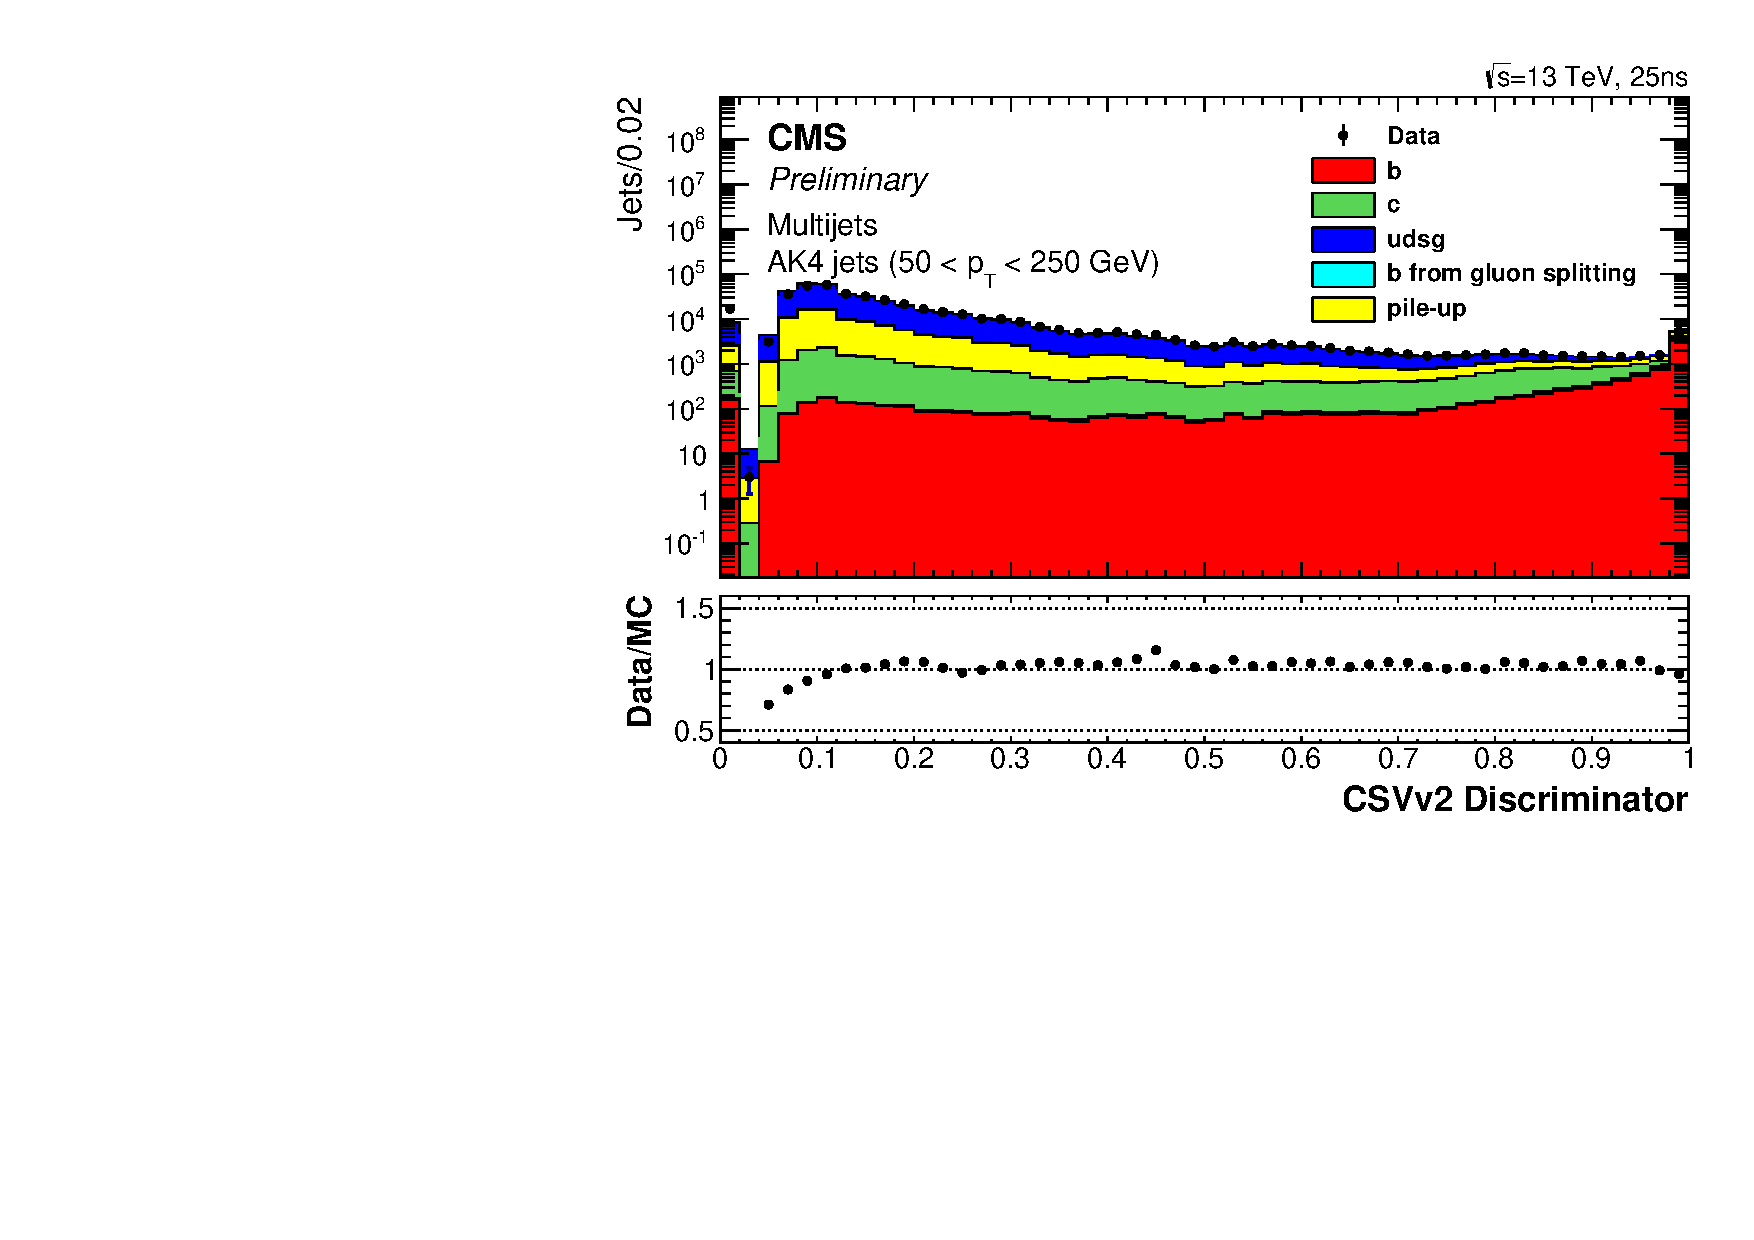
\includegraphics{figs/data-mc/ak4_pfjets_CSVIVF_Log.pdf}
\caption{The distribution of the CSVv2 algorithm's discriminator for multijet events, for $50\GeV < \pT < 250\GeV$, at $\sqrt{13\TeV}$, where the jets have been reconstructed with the anti-\kt algorithm with $R = 0.4$~\cite{CMS:2016kkf}. T}
\label{fig:bTagDiscriminator}
\end{figure}

\subsection{Missing Transverse Energy}\label{subsec:objReco-MET}
Particles which only weakly interact with matter, such as neutrinos and some hypothesised BSM particles, escape the detector without being directly observed, but can be inferred from considering the conservation of the transverse momentum of the event.
Therefore, the missing energy in the plane transverse to the beam line, $\overrightarrow{\MET}$, is defined as the negative vector sum of the transverse momentum in the end:

\begin{equation}
\overrightarrow{\MET} = - \sum \overrightarrow{\pT} \;
\label{eq:MET}
\end{equation}

There are several different algorithms, using differing variables and techniques, which are used in CMS analyses to determine \MET.
PF \MET, producing using the PF particles, is used in this analysis because of its high performance with \emph{Type-I} \MET corrections applied~\cite{CMS:2016ljj}.
This correction applies the jet energy corrections discussed in Section~\ref{subsubsec:JECs} to the PF jets with $\pT >15\GeV$ which are used in calculating the \MET.

The Type-I corrections become unreliable for jets with $\pT <15\GeV$, so \emph{Type-II} \MET corrections are derived from the \emph{unclustered} energy deposits.

Given that the event selection for the analysis presented in this thesis uses jets with $\pT > 30\GeV$, the \emph{Type-II} corrections (discussed in detail in~\cite{Chatrchyan:2011tn}) applied to jets with $\pT < 15\GeV$ is not considered.
